\documentclass[10pt,a4paper]{article}
\usepackage[utf8]{inputenc}
\usepackage{amsmath}
\usepackage{amsfonts}
\usepackage{amssymb}

\usepackage{pdflscape}

\usepackage{float}
\usepackage[table,xcdraw]{xcolor} %para usar tablas con color de fondo en las celdas
\usepackage{hyperref} %para poder poner enlaces
\usepackage{listings} %para insertar código
\usepackage{tikz}%para pintar las redes neuronales
%\usepackage{color} %para poder definir y usar colores
\usepackage{soulutf8} %para hacer los subrayados

\author{\textbf{Gustavo Rivas Gervilla}}
\title{\textcolor{deepblue}{\textbf{Titanic. Competición Kaggle.}}}
\date{}

%Configurando lstlisting para mostrar código Python con algún 	 de colores (copiado de http://tex.stackexchange.com/questions/83882/how-to-highlight-python-syntax-in-latex-listings-lstinputlistings-command) ------------------------------
% Custom colors
\definecolor{deepblue}{rgb}{0,0,0.5}
\definecolor{rblue}{rgb}{0.2,0.6,1}
\definecolor{deepgreen}{rgb}{0,0.5,0}
\definecolor{light-gray}{gray}{0.85}
\definecolor{comment-gray}{gray}{0.65}
\definecolor{light-blue}{rgb}{0.6,1,0.8}
\definecolor{light-yellow}{rgb}{1,1,0.6}

% Default fixed font does not support bold face
\DeclareFixedFont{\ttb}{T1}{txtt}{bx}{n}{8} % for bold
\DeclareFixedFont{\ttm}{T1}{txtt}{m}{n}{8}  % for normal

%Configuración de los listings
\lstset{
	language=Python,
	basicstyle=\ttm,
	otherkeywords={self},             % Add keywords here
	keywordstyle=\ttb\color{deepblue},
	emph={MyClass,__init__},          % Custom highlighting
	emphstyle=\ttb\color{deepred},    % Custom highlighting style
	stringstyle=\color{deepgreen},
	frame=tb,                         % Any extra options here
	showstringspaces=false,            % 
	commentstyle=\ttm\color{comment-gray}, % Custom comment style
}
%--------------------------------------------------------------------------------

\newcommand{\emp}[1]{\sethlcolor{light-yellow}\hl{#1}} %Comando para poner código inline
\newcommand{\code}[1]{\sethlcolor{rblue}\hl{\texttt{#1}}} %Comando para poner código inline
\newcommand{\archive}[1]{\sethlcolor{light-blue}\hl{\texttt{#1}}} %Comando para resaltar nombres de archivos
\renewcommand\tablename{Tabla} %Cambiar el nombre de las tablas
\renewcommand\figurename{Figura} %Cambiar el nombre de las tablas
\renewcommand{\contentsname}{Índice} %Cambiar el nombre de la ToC

\usepackage{pdfpages}

\begin{document}
\maketitle

\begin{center}
  \textbf{Nombre del equipo: }Gustavo Rivas Gervilla\\
  \textbf{Ranking global: }TODO\\
  \textbf{Puntuación: }TODO
\end{center}

\newpage

\tableofcontents

\newpage

\section{Introducción}

En este trabajo se va a trabajar con el dataset del Titanic, un conjunto de datos en el que se plantea un \textbf{problema de clasificación}, dadas una serie de características de un pasajero, que enumeraremos en la siguiente sección, se tendrá que decidir si el pasajero sobrevivió o no a la catastrofe. En primer lugar, como toma de contacto con el dataset y también para tomar algunas ideas que aplicar al conjunto de datos, se han realizado dos tutoriales con planteamientos similares, ambos realizan un preprocesamiento parecido a los datos y emplean Random Forest como algoritmo final de clasificación, después de probar otros modelos como puede ser uno basado en un árbol de decisión o simplemente suponer que todas las mujeres sobrevivieron y que todos los hombres perecieron. La realización de estos dos tutoriales se adjunta en esta memoria a modo de apéndices.\\

\section{Exploración de datos} \emph{Ver archivo \archive{exploracion.Rmd}}\\

En primer lugar vamos a presentar el conjunto de datos que tenemos, disponemos de 891 instancias en el conjunto de entrenamiento y 418 en el conjunto de test. Estas instancias presentan el siguiente conjunto de atributos:

\begin{enumerate}
\item \textbf{PassengerId: } identificador del pasajero.
\item \textbf{Pclass: } la clase en la que embarcó.
\item \textbf{Name:} el nombre del pasajero.
\item \textbf{Sex: } sexo del pasajero.
\item \textbf{Age: } edad del pasajero.
\item \textbf{SibSp: } número de hermanos/esposos/esposas del pasajero que viajaban también a bordo.
\item \textbf{Parch: } número de padres/hijos del pasajero que viajaban también a bordo.
\item \textbf{Ticket: } número o identificador del ticket de embarque del pasajero.
\item \textbf{Fare: } lo que pagó el pasajero por su pasaje.
\item \textbf{Cabin: } camarote(s) en el(los) que viajó el pasajero.
\item \textbf{Embarked: } puerto desde el que embarcó. C = Cherbourg, Q = Queenstown, S = Southampton.
\item \textbf{Survived: } el pasajero murió (0) o sobrevivió (1). La variable a predecir y que por tanto no está presente en las intancias del conjunto de test.
\end{enumerate}

Lo primero que hemos hecho ha sido estudiar si contábamos con valores perdidos. Gracias a los tutoriales notamos que hay algunos atributos que, si bien no presentan valores perdido (\textbf{NA}), contienen una cadena vacía lo que se podría considerar también un valor perdido, y por lo tanto esto también se tendrá en cuenta en la fase de preprocesamiento. Tras este análisis vemos que la mayoría de valores perdidos están en el atributo \textbf{Age}, también hay algún valor perdido en el \textbf{Embarked} y muchos valores perdidos para el atributo \textbf{Cabin} (señalar aquí que en R es mejor emplear los operandos condiciones \texttt{\&} y \texttt{|}, en lugar de \texttt{\&\&} o \texttt{||}, ya que con estos obtenemos resultados incorrectos).\\\\

De hecho en ambos conjuntos, para el atributo \textbf{Cabin} tenemos aproximadamente un 78\% de valores perdidos, lo cual es una cantidad muy elevada. Esto nos lleva a dudar si será útil crear una variable que contenga la cubierta en la que viajó el pasajero. Tratar de imputarla de algún modo no parece que vaya a dar un buen resultado al tener tan poca información para dicho atributo.\\

Vamos a ver ahora la primera gráfica sobre nuestro conjunto de datos, lo que vamos a reflejar en esta gráfica es el desequilibrio entre las dos clases (549 muertos y 342 sobrevivientes), aunque no se trata de un desequilibrio demasiado grande lo trataremos en la fase de preprocesamiento y trataremos de comparar distintas técnicas de balanceo de clases según su rendimiento para un algoritmo determinado:

\begin{figure}[H]
  \centering
  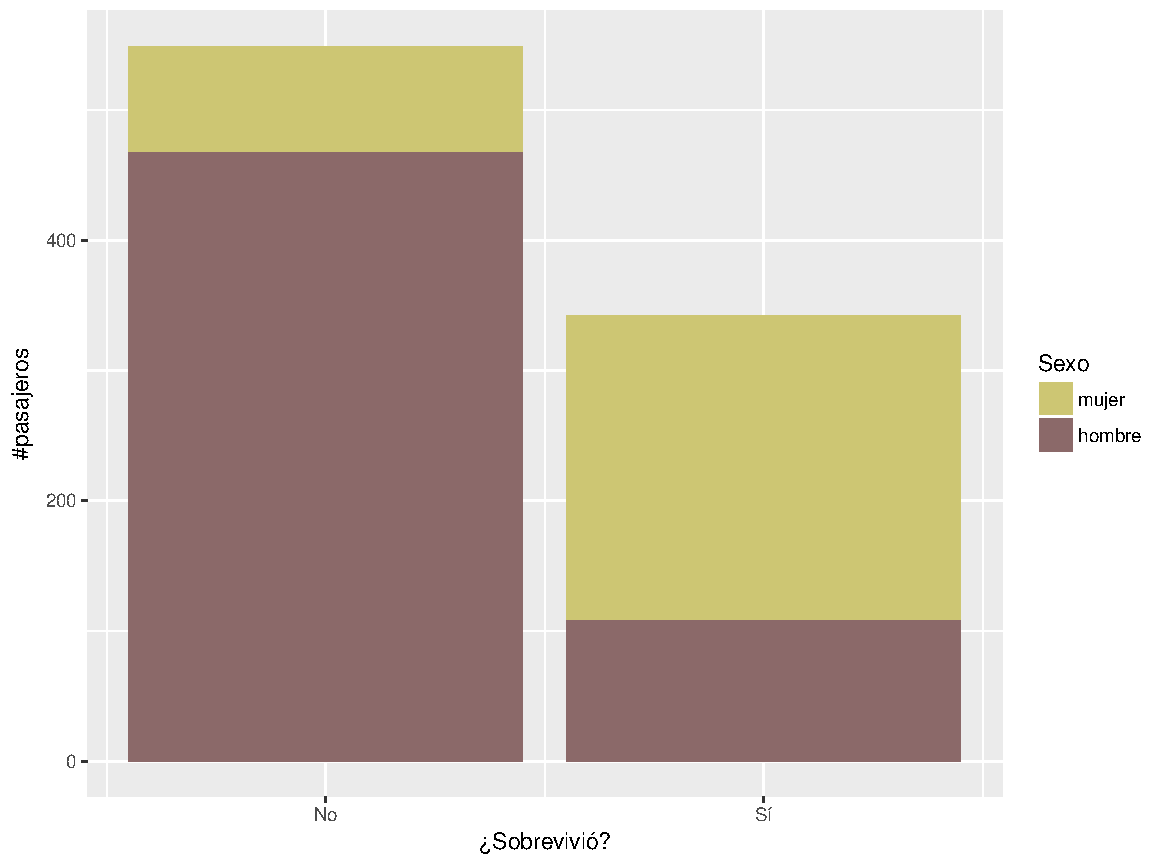
\includegraphics[width=\textwidth]{imgs/imbalanced.pdf}
  \caption{Desbalanceo entre clases}
\end{figure}

En la gráfica anterior también mostramos en qué proporción sobreviven hombres y mujeres en el conjunto de entrenamiento. Como podemos ver son las mujeres las que en su mayoría sobrevivieron mientras que los hombres tuvieron menos posibilidades, recordemos que durante el accidente del Titanic se estableció la política de evacuar a mujeres y niños en primer lugar con lo que esta gráfica parece acorde a ello. Este hecho nos lleva, en el tutorial de Trevor Stephens, a plantear el modelo sexista.

\section{Preprocesamiento} \emph{Ver archivo \archive{preprocesamiento.Rmd}}\\

TODO Explicar las tantas de prepro.

\subsection{Preprocesamiento básico}


Lo primero que hemos hecho ha sido \emp{fabricar una nueva variable que recoge el título de cada pasajero}, para ello hemos extraído este título del nombre de cada pasajero. El título podría darnos información de la clase social del pasajero y quizás aquellos pasajeros de mayor estatus tuvieron mayor posibilidad de ser evacuado. El \textit{problema} que presenta esta variable es que presenta muchos valores distintos a lo largo de los \textit{datasets} con lo cual lo que hemos hecho es agrupar distintos títulos es uno solo.\\

Muchos de estos títulos son equivalente, con lo cual tener una granularidad tan alta en una variable quizás lo único que haría sería provocar que nuestros modelos funcionasen peor al introducir una componente de sobreajuste en los mismo.\\

A continuación lo que hemos hecho ha sido, combinando la variable anterior con el apellido de cada pasajero, se \emp{fabrica una nueva variable que se puede ver como un identificador para la familia abordo del pasajero}. Esta variable tiene sentido ya que, si bien pensamos que familias demasiado grandes pudieron tener más problemas para ser evacuadas, puede que unas familias, por su estatus, tuviesen más fácil el ser evacuadas. Combinamos las dos variables y no usamos únicamente el apellido para intentar no mezclar personas de distintas familias dentro del mismo identificador.\\

No obstante, para que esta variable no tenga una granularidad muy elevada (por ejemplo el Random Forest del paquete \code{randomForest} no admite variables de tipo factor con más de 32 niveles), hemos asignado todas las familias con 2 miembros o menos en un mismo identificador \code{'Small'}, esto concuerda con lo que vimos en la sección de exploración, aquellos que viajaban solos tenían más posibilidades de morir, aunque quizás sí que penaliza a las familias de dos miembros.\\

A continuación lo que hacemos es \emp{imputar los valores perdidos para el atributo \textbf{Embarked}}, esto sólo ocurre en dos instancias del conjunto de datos, y dado que las dos pasajeras no cuenta de familiares a bordo con los que poder deducir el puerto desde el que embarcaron, ambas pagaron lo mismo por su pasaje(80\$) en primera clase y Southhampton es el puerto más frecuente, además de que la media de la tarifa de embarque en primera clase desde este puerto es de aproximadamente 72\$, decidimos asignarle a ambas pasajeras dicho puerto. En el tutorial de Megan Risdal en cambio se le asigna el puerto \code{C} que tiene una media de precio de 90\$ y es menos frecuente que el \code{S}. Nosotros hemos optado por la idea que se da en el tutorial de Trevor Stephens. De todos modos estamos hablando de una decisión que sólo afecta a dos instancias del conjunto completo de datos con lo que no es algo crítico.\\

Algo más simple fue la decisión para \emp{imputar el único valor perdido que tenemos para el atributo \textbf{Fare}}, lo único que hemos hecho ha sido asignarle al pasajero del que no conocemos la tarifa que pagó la media de lo que pagaron otros pasajeros con sus mismas características (embarcaron desde el mismo puerto y en la misma clase que él).\\

Ahora lo que vamos a hacer va a ser \emp{imputar los valores perdidos para el atributo \textbf{Age}}, para este atributo sí que tenemos más valores perdidos, 263, con lo cual vamos a emplear una técnica algo más sofisticada para imputar estos valores perdidos, vamos a emplear el método Random Forest haciendo uso del método \code{myce}. En este procedimiento excluimos algunas variables para predecir la edad ya que no creemos que aporten información relevante para la edad del pasajero, como son la familia a la que pertenece el pasajero o el identificador de su ticker de embarque. También ignoramos el atributo \code{Survived} ya que las instancias del conjunto de test no disponen de tal información.\\

Una vez que tenemos todos las edades de los pasajeros pasamos a \emp{crear una variable que indique si un pasajero es adulto o no}, considerando a una persona adulta a partir de los 18 años. TODO explicar por qué creo esta variable. Llamaremos a este nuevo atributo \code{Child}.\\

Finalmente se ha \emp{creado una variable que indica si un pasajero es madre o no}, esto lo hacemos porque parece lógico pensar que aquellas mujeres acompañadas de niños, probablemente sus hijos, tuviesen mayor preferencia a la hora de ser evacuada.

Señalar que en un de los tutoriales que se han consultado durante la realización de esta práctica se procesa la variable \code{Cabin} para obtener la cubierta en la que viajó este pasajero, este dato puede ser muy interesante ya que según la localización del pasajero en el barco sus posibilidades de sobrevivir pudieron ser mayor o menores. Sin embargo, dado que el número de valores perdidos es muy elevado, se ha decidido no crear esta nueva variable, ya que la imputación podría resultar muy mala al haber más valores perdidos que presentes, el análisis de esta variable se verá como trabajo futuro.

\subsection{Eliminando ruido}

\subsection{Balanceando las clases}

\section{Técnicas de clasificación}

\section{Presentación y discusión de resultados}

\section{Conclusiones y trabajo futuro}

TODO la selección de características parece que da muy buenos resultados.
TODO probar con otros agrupamientos de títulos.
TODO estudiar la creación de la variable con la cubierta en la que estaba el pasajero.
TODO tunear xgboost
TODO redes neuronales

\begin{landscape}
\section{Listado de soluciones}
\pagestyle{empty}

\begin{table}[H]
\centering
\caption{Listado de resultados}
\label{my-label}
\begin{tabular}{|c|l|c|c|c|c|}
\hline
\rowcolor[HTML]{C0C0C0} 
Nº                                & \multicolumn{1}{c|}{\cellcolor[HTML]{C0C0C0}\textbf{Descripción. preprocesamiento}}                                                                                                                                                                                         & \textbf{Alg. y soft. empleados}        & \textbf{\begin{tabular}[c]{@{}c@{}}Acierto\\ train\end{tabular}} & \textbf{\begin{tabular}[c]{@{}c@{}}Acierto\\ test\end{tabular}} & \textbf{Ranking} \\ \hline
\textbf{1}                        & \begin{tabular}[c]{@{}l@{}}El preprocesamiento de Megan Risdal:\\ - Extracción del título.\\ - Tamaño de famila e id de la misma.\\ - Imputación de valores perdidos, algunos con mice.\\ - Variables indicando si el pasajero es mayor de edad y si es madre.\end{tabular} & Random Forest del paquete randomForest & 0.8349884                                                        & 0.80383                                                         & 1034             \\ \hline
\rowcolor[HTML]{9AFF99} 
\textbf{2}                        & \begin{tabular}[c]{@{}l@{}}El preprocesamiento de Trevor Stephens:\\ - Variable indicando si es un adulto o no.\\ - Título del pasajero.\\ - Tamaño de la famila e id de la misma.\\ - Imputación de valores perdidos, árbol de decisión para la edad.\end{tabular}         & Random Forest del paquete party        & 0.8316678                                                        & 0.81340                                                         & 429              \\ \hline
\textbf{3}                        & El mismo de el tutorial de Stephens.                                                                                                                                                                                                                                        & rpart                                  & 0.8305505                                                        & 0.79426                                                         & 1469             \\ \hline
\textbf{4}                        & El mismo de el tutorial de Stephens.                                                                                                                                                                                                                                        & xgboost del paquete xgboost            & 0.8372921                                                        & 0.81340                                                         & 421              \\ \hline
\textbf{5}                        & El mismo de el tutorial de Stephens.                                                                                                                                                                                                                                        & Ensamble de rpart + xgboost + cforest  &                                                                  & 0.80861                                                         & 537              \\ \hline
\textbf{6}                        & El mismo de el tutorial de Stephen + down sampling.                                                                                                                                                                                                                         & cforest                                & 0.820283                                                         & 0.79426                                                         & 1691             \\ \hline
\textbf{7}                        & El mismo de el tutorial de Stephen + down sampling.                                                                                                                                                                                                                         & rpart                                  & 0.8202832                                                        & 0.78947                                                         & 2096             \\ \hline
\textbf{8}                        & El mismo de el tutorial de Stephen + down sampling.                                                                                                                                                                                                                         & xgboost                                & 0.8202832                                                        & 0.77990                                                         & 3186             \\ \hline
\textbf{9}                        & El mismo de el tutorial de Stephen + up sampling.                                                                                                                                                                                                                           & cforest                                & 0.8123288                                                        & 0.78469                                                         & 2720             \\ \hline
\textbf{10}                       & El mismo de el tutorial de Stephen + up sampling.                                                                                                                                                                                                                           & rpart                                  & 0.8132586                                                        & 0.73684                                                         & 6204             \\ \hline
\textbf{11}                       & El mismo de el tutorial de Stephen + up sampling.                                                                                                                                                                                                                           & xgboost                                & 0.8250809                                                        & 0.76555                                                         & 5044             \\ \hline
\multicolumn{1}{|l|}{\textbf{12}} & El mismo de el tutorial de Stephen + SMOTE.                                                                                                                                                                                                                                 & cforest                                & 0.9132704                                                        & 0.80383                                                         & 1007             \\ \hline
\multicolumn{1}{|l|}{\textbf{13}} & El mismo de el tutorial de Stephen + SMOTE.                                                                                                                                                                                                                                 & rpart                                  & 0.8923114                                                        & 0.77512                                                         & 3606             \\ \hline
\multicolumn{1}{|l|}{\textbf{14}} & El mismo de el tutorial de Stephen + SMOTE.                                                                                                                                                                                                                                 & xgboost                                & 0.9108267                                                        & 0.79426                                                         & 1722             \\ \hline
\multicolumn{1}{|l|}{\textbf{15}} & El mismo de el tutorial de Stephen + SMOTE + IPF.                                                                                                                                                                                                                           & cforest                                & 0.9994536                                                        & 0.77512                                                         & 3606             \\ \hline
\multicolumn{1}{|l|}{\textbf{16}} & El mismo de el tutorial de Stephen + SMOTE + IPF.                                                                                                                                                                                                                           & rpart                                  & 0.9983636                                                        & 0.77033                                                         & 4178             \\ \hline
\multicolumn{1}{|l|}{\textbf{17}} & El mismo de el tutorial de Stephen + SMOTE + IPF.                                                                                                                                                                                                                           & xgboost                                & 0.9978187                                                        & 0.77033                                                         & 4178             \\ \hline
\end{tabular}
\end{table}

\end{landscape}

\appendix

\section{Tutorial ``Exploring Survival on the Titanic'' de Megan Risdal}

%\includepdf[pages=-]{StephensTitanicTutorial}

A modo de introducción tanto al dataset como a la plataforma Kaggle vamos a realizar este tutorial que nos servirá para dar una primera solución al problema que se nos plantea con este dataset. También, y simplemente por conocer esta herramienta, se ha optado por realizar este tutorial desarrollando un aplicación web Shiny. El fichero tiene extensión de Rmarkdown, algo que ya he usado, con lo cual no debería ser muy complicado usar esta utilidad que ofrece Rstudio.

\subsection{Preprocesamiento}

Lo primero que observamos es el uso de la función \code{bind\_rows} del paquete \code{dplyr}, lo que hacemos con esta función es unir los datasets de train y test en uno solo, la diferencia entre esta función y usar por ejemplo \code{rbind} es que nos facilita el trabajo, ya que mientras que \code{rbind} nos da un error al no tener ambos datasets el mismo número de columnas (el conjunto de test no contiene la clase a la que pertenece cada una de las instancias ya que es lo que hemos de predecir de cara a la competición), con \code{bind\_rows} lo que hace es unir ambos e insertar \textbf{NA} en aquellos atributos que no están presentes en el dataset de test, la clase de los pasajeros.\\

En el tutorial realiza una pequeña exploración sobre el conjunto total de instancias del problema haciendo uso de la función \code{str} aunque esto no nos aporta información acerca de la semántica de cada uno de los atributos del dataset, estos son los siguientes:

\begin{enumerate}
\item Survived: la clase a predecir. Sobrevivió (1) o murió (0).
\item Pclass: la clase del pasaje.
\item Name: el nombre del pasajero.
\item Sex: sexo del pasajero.
\item Age: edad del pasajero.
\item SibSp
\item Parch
\item Ticket
\item Fare: 
\item Cabin: número de camarote.
\item Embarked: puerto en el que embarcó.
\end{enumerate}

\subsection{Subiendo resultados a Kaggle}

A modo de ejercicio lo que he hecho ha sido generar simplemente una predicción completamente aleatoria, de este modo podremos testear rápidamente el sistema de subida a la plataforma Kaggle y además tener un punto de referencia más para comparar los distintos experimentos que realicemos. Con esta predicción hemos obtenido un score de \textbf{0.43541}. Observemos que hemos puesto el atributo \code{quote} de la función \code{write.csv} de modo que el nombre de las columnas del dataset se introduzcan sin ir entre comillas dobles, de otro modo Kaggle no aceptaría el submisión.

Tras el tutorial de Riscal pos \textbf{989} accuracy \textbf{0.80383}

Tras aplicar Xgboost al dataset de Riscal \textbf{0.77990}.

\end{document}